% Written by Kamila Larripa, July 2020 for Math 102
\documentclass[12pt]{amsart}
\usepackage{amssymb, latexsym,xspace}
\usepackage[pdftex]{graphicx}

%%%%%%%%%%%%%%%%%%%%%%%
%
% Change course, date, etc. here and the 
% header will be automatically generated.
%
%%%%%%%%%%%%%%%%%%%%%%%
\newcommand{\class}{Math 102}
\newcommand{\term}{Precalculus}
\newcommand{\quiztitle}{Problem Set 1: Lines, Circles, Distance and Midpoint Formula, Functions and Domains}
%%%%%%%%%%%%%%%%%%%%


%%%%%% Small margin to leave room for students' work %%%%%%%
\usepackage[margin=0.75in,top=0.5in,
            nohead,
            pdftex]{geometry}

%%%%%% Various PDF commands; generally not needed in a quiz %%%%%%%
\usepackage[pdftex, colorlinks=true,
            linkcolor=blue, citecolor=blue,
            urlcolor=blue, letterpaper,
            pdftitle={},
            pdfpagemode=None]{hyperref}

%%%%% spread the lines out a bit.
\pagestyle{plain}
\linespread{1.3}
\parindent 0ex

\begin{document}
%%%%%%%%% Header %%%%%%%%%%%
\textbf{\class \xspace\xspace \term \xspace\xspace - \quiztitle\\}
%\quizdate\xspace\xspace - \timelimit \hspace{1.5in} Name: }\\
\rule[1ex]{\textwidth}{.1pt}


\vspace{1em}
%This problem set covers topics from section 2.1, 2.2, 2.3.  Topics include lines, circles, the distance and midpoint formula, functions, and domains of functions.

\begin{enumerate}

\item Consider the points $(-1,2)$ and $(0,-2)$.
\begin{enumerate}
     \item Plot and label these points in the $x$-$y$ plane.
     \item Find the slope of the line connecting these points.
     \item Write the equation of the line that goes through these points in point-slope form.
     \item Write the equation of the line that goes through these points in slope--intercept form.
     \item Sketch the line and label the $y$-intercept.
    \end{enumerate}

%\item Repeat the steps above for the points $(1,3)$ an $(2,3)$.
\item Repeat the steps above for the points $(\frac{2}{3},-1)$ an $(-\frac{1}{3},-2)$.
%\item Repeat the steps above for the points $(3,2)$ an $(5,2)$. 

 \item Consider the line $y=-2x+5$.
  \begin{enumerate}
     \item Determine whether the point $(2,1)$ lies on the graph of the line.  Approach this problem two ways-- use the equation and also use your graph by plotting the point.
     \item Determine whether the point $(3,-1)$ lies on the graph of the line.
     \item Determine whether the point $(3,-2)$ lies on the graph of the line.
     %\item Determine whether the point $(2,1)$ lies on the graph of the line.
      \end{enumerate}

\item Consider the equation $-3x + 6y -2 = 0$.
 \begin{enumerate}
     \item Rewrite this equation in slope-intercept form.
      \item What is the slope of this line?
     \item What is the $y$-intercept (give as a point)?
     \item What is the $x$-intercept (give as a point)?  Hint: to find an $x$-intercept, set $y=0$ and solve for $x$.
     \item Sketch the line.
     \item What observations can you make about the general form of the equation of a line?  For example, what are the powers of $x$ and $y$ terms for equations of lines?
      \end{enumerate}

%\item Consider the equation $3(x-2) + 4y -7 = 0$ and repeat the steps in the problem above.



\item Consider the following graph.  Write the equation of the line in slope-intercept form.
\begin{figure}[h!]
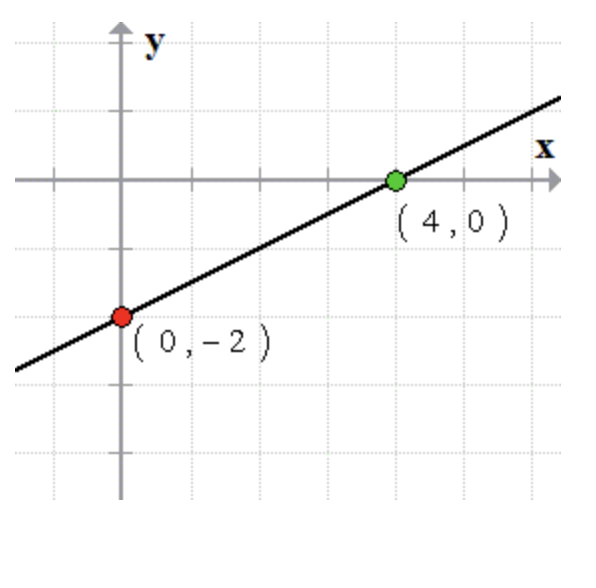
\includegraphics[width=6cm]{line.png}
\end{figure}
      
      
\item Consider the line $x=5$.
 \begin{enumerate}
     \item List any two points which lie on this line.
      \item In general, if a point is on this line, what is its $x$-coordinate? 
     \item What is the slope of this line?
     \item We have defined slope to be ``rise over run.''  For the two points you selected, what is the rise?  What is the run?
     \item Write a short explanation for why a number divided by zero is undefined.  Hint: Feel free to use google.  Both Wikipedia and Khan Academy have explanations.
      \item Sketch the line.
      \end{enumerate}


%\item Consider the line $y=-3$.
% \begin{enumerate}
%     \item List any two points which lie on this line.
%      \item In general, if a point is on this line, what is its $y$-coordinate? 
%     \item What is the slope of this line?
%     \item We have defined slope to be ``rise over run.''  For the two points you selected, what is the rise?  What is the run?  Does this match up with the slope you found?  
%      \item Sketch the line.
%      \end{enumerate}
%
      
\item Consider the line $y=-\frac{1}{3}x-1$.
 \begin{enumerate}
     \item Write the equation of the line parallel to the given line and passing through the point $(3,2)$.  Give your equation in slope-intercept form.
      \item Sketch both lines.    
       \item What is the only difference between the equations for each line?
      \end{enumerate}
      

\item Consider the line $y=2x-1$.
 \begin{enumerate}
     \item Write the equation of the line perpendicular to the given line and passing through the point $(-2,1)$.  Give your equation in slope-intercept form.
      \item Sketch both lines.    
       \item Where do the lines intersect?  Hint: set the equations equal to each other and solve for $x$.  Then use this $x$ value to solve for $y$.
      \end{enumerate}
      

%\Large{\textbf{Challenge Problems}}

%\item The vertices of a right triangle are at points $(-3,4)$, $(-3,-4)$ and $(7,-4)$.
% \begin{enumerate}
%     \item Sketch this triangle and label the vertices.
%      \item Explain how you know the point $(2,0)$ lies on the hypotenuse of the triangle.
%  \end{enumerate}
%

\item Consider a line, $y=2x+1$.  
 \begin{enumerate}
     \item If the line is reflected across the $y$-axis, find its equation.  Sketch both lines.  How did the $y$ intercept change with the reflection?  How did the slope change with the reflection?
      \item If the line is reflected across the $x$-axis, find its equation.  Sketch both lines.  How did the $y$ intercept change with the reflection?  How did the slope change with the reflection?
      \item Can you make any generalizations about a line of the form $y=mx+b$ and the equations of the reflections above?  Hint: it might help to do a few more concrete examples.
  \end{enumerate}
  
  
  \item A line with slope $-3$ passes through the points $(-8,p)$ and $(2,3p)$.
 \begin{enumerate}
     \item Find $p$.
      \item Write the equation of this line in slope-intercept form.
      \item Sketch this line.
  \end{enumerate}
  
 \item Graph a family of lines  of the form $y=3x+c$ on the same $x$-$y$ plane where $c$ is any real number.  Describe the pattern of the graph.  How does changing $c$ change the graphs of the lines?  Hint: choose a few values of $c$ and graph those lines.  For example, you might sketch $y=3x+1$, $y=3x+2$, $y=3x-10$.
  
\item Graph a family of lines  of the form $y=dx+1$ on the same $x$-$y$ plane where $d$ is any real number.  Describe the pattern of the graph.  How does changing $d$ change the graphs of the lines?  Now check your intuition using this Desmos application which has a slider for the parameters $m$ and $b$ for lines of the form $y=mx+b$: https://www.desmos.com/calculator/wuxkicjcre


\item Consider the points $(2,3)$ and $(0,6)$.
\begin{enumerate}
     \item Plot and label these points in the $x$-$y$ plane.
     \item Find the slope of the line connecting these points.
     \item Find the distance between the points.
     \item Find the midpoint of the line segment connecting these points.  Label the midpoint on your sketch.
    \end{enumerate}

 \item Find a point of the form $(2a,a)$ in the third quadrant such that the distance from this point to $(1,3)$ is $5$.  Hint:  You might start by writing the distance formula for the two points and setting it equal to $5$.

\item Consider the circle with equation $x^2+y^2+8x-6y+16=0$.
\begin{enumerate}
\item Complete the square to put this equation in standard form ($(x-h)^2+(y-k)^2=r^2$).
\item What is the center?
\item What is the radius?
\item Sketch the circle.
\item Is this a function?
\end{enumerate}

%\item Consider the following mapping.  Is it a function?  Why or why not?
%\begin{figure}[!h]
%\includegraphics[width=3cm]{function.png}
%\end{figure}

%\pagebreak

\item Consider the following mapping.  Is it a function?  Why or why not?
\begin{figure}[!h]
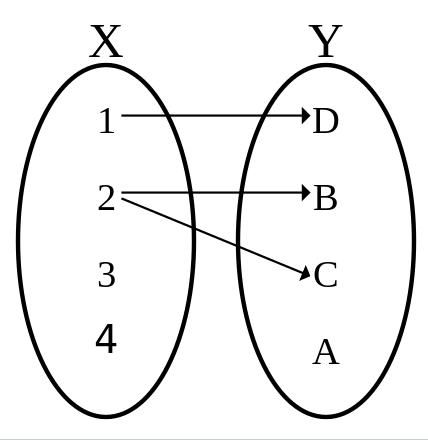
\includegraphics[width=3cm]{notfunction.png}
\end{figure}
      



\item Let $f(x)=8-x^2$.  Fill out the following table by evaluating the function.
\begin{center}
 \begin{tabular}{||c c||} 
 \hline
 $x$ & $f(x)$ \\ [0.5ex] 
 \hline\hline
 -2 &   \\ 
 \hline
 -1 &   \\
 \hline
 0 &  \\
 \hline
 1 &   \\
 \hline
 2 &  \\
 \hline
  $apple$ &  \\ 
 \hline
  $2+h$ & \\
   \hline
\end{tabular}
\end{center}      

\item Consider $f(x)=2x+1$.
\begin{enumerate}
\item
Fill out the following table (I did the first row as an example):
\begin{center}
 \begin{tabular}{||c c c c||} 
 \hline
 $x$ & $f(x)$  &$f(x+2)$ & $f(x)+3$\\ [0.5ex] 
 \hline\hline
\textcolor{blue} {1} & $2(\textcolor{blue}{1})+1 =3$ & $2(\textcolor{blue}{1}+2)+1=7$ & $2(\textcolor{blue}{1})+1 +3=6$ \\ 
 \hline
 2 & & &  \\
 \hline
 3 & & &  \\
 \hline
 4 & & &  \\
    \hline
\end{tabular}
\end{center}      

\item Sketch $f(x)$.   Label the four points in your table on the graph.
\item Sketch $f(x+2)$.  Label the four points in your table on the graph.  How does this sketch relate to the sketch of $f(x)$?
\item Sketch $f(x)+3$.    Label the four points in your table on the graph.  How does this sketch relate to the sketch of $f(x)$?
\item Can you make a guess about how the addition of constants inside and outside the function alters the graph?  For example, $f(x+a)$ does what to a graph?  And $f(x) + b$ does what?
\end{enumerate}

\item Sketch the domain of each function on the real number line.  Give the domain in \textbf{interval notation} of the following functions.
\begin{enumerate}
\item $f(x)=\sqrt{x-7}$
\item $f(x)=\frac{1}{x-4}$
\item $f(x) = \frac{2x-3}{3x+5}$
\item $f(x) = \sqrt{x-5} + \frac{x+1}{x-10}$ Hint: you might consider the domain of each term separately, then look for the intersection.
\end{enumerate}

\item REFLECTION AND CONSOLIDATION (Hint: this will form part of a study guide for your first exam!)
\begin{enumerate}
\item Summarize the main ideas/formulas you used for this problem set.  You can list formulas, bullet-out phrases, write a paragraph, draw sketches, or answer this question in any way that makes sense to you.
\item What three problems were the most challenging for you?  After deciding, look at your solutions carefully, and write a short explanation of what you found challenging and how you overcame this challenge in your problem solving.  For example, did you find a simpler problem about the same topic?  Did you guess and check?  Did you graph with technology?
\item Write three potential test questions on the topics covered in this problem set.
\end{enumerate}


\end{enumerate}


\end{document}